\documentclass[12pt, a4paper]{article}
\usepackage{amsmath, amsfonts, amssymb}
\usepackage{graphicx}
\usepackage{booktabs}
\usepackage{geometry}
\usepackage{hyperref}
\usepackage{fancyhdr}
\usepackage{cite}
\usepackage{caption}
\usepackage{subcaption}
\usepackage{float}
\usepackage{tabularx} % 用于自适应宽度表格
\usepackage{array}    % 用于控制列的对齐方式
\usepackage{indentfirst} % 用于强制首段缩进

% Page margin settings
\geometry{left=2.5cm, right=2.5cm, top=2.5cm, bottom=2.5cm}

% 设置段落首行缩进为2个字符宽度
\setlength{\parindent}{2em}

% Header and footer settings: remove header, page number at footer center
\pagestyle{fancy}
\fancyhf{} % Clear header and footer
\renewcommand{\headrulewidth}{0pt} % Remove header line
\cfoot{\thepage} % Page number at footer center

\title{\textbf{Death Risk Prediction and Risk Factor Analysis of Heart Failure Patients Based on Clinical Data and Machine Learning}}


\begin{document}
\date{}
\maketitle

\section*{Abstract}
The clinical outcomes of patients with Heart Failure (HF) are influenced by the complex interplay of various demographic characteristics, laboratory test indicators, and cardiac function metrics. To explore a refined mortality risk assessment method driven by clinical data, this study constructed and compared four classification models: Logistic Regression (LR), Random Forest (RF), Extreme Gradient Boosting (XGBoost), and Multi-Layer Perceptron (MLP), based on the publicly available Heart Failure Clinical Records dataset. The study first conducted descriptive statistics, missing value and outlier tests, correlation analysis, and feature preprocessing; subsequently, it identified candidate clinical indicators closely related to mortality outcomes by combining statistical hypothesis testing and tree model feature importance analysis; finally, through stratified training and testing set splitting, five-fold cross-validation, and independent test set evaluation, the classification performance of different models was compared, and a comprehensive evaluation was conducted using the ROC curve, area under the curve (AUC), and multivariate classification metrics.

The dataset contains a total of 299 patient records (203 cases without death events and 96 cases with death events). Experimental results showed that serum creatinine, ejection fraction, and age were the most prominent in statistical tests and random forest feature importance analysis. Different models exhibited distinct characteristics in classification performance, among which the Random Forest achieved relatively higher Recall and F1 scores on the test set. The early warning framework constructed in this study demonstrates the potential of machine learning in heart failure risk stratification. The results are primarily intended for methodological exploration and educational demonstration, and do not constitute clinically validated diagnostic recommendations.

\noindent\textbf{Keywords: }Heart Failure; Machine Learning; Mortality Risk Prediction; Risk Factors; Logistic Regression; Random Forest; XGBoost; Multi-Layer Perceptron


\newpage

\section{Introduction}
Heart Failure (HF) is the terminal stage of various cardiovascular diseases, characterized by extremely high disability and mortality rates. The prognosis of HF patients is jointly regulated by age, cardiac systolic function, renal function status, and multiple metabolic indicators. Traditional clinical risk assessment tools mostly rely on linear or proportional hazard assumptions, and their generalization capabilities may be limited when facing highly non-linear, multi-variable synergistic complex clinical data. With the popularization of Electronic Health Records (EHRs), utilizing structured clinical data combined with Machine Learning (ML) algorithms for risk stratification can uncover underlying pathophysiological patterns and provide auxiliary support for clinical decision-making.

In data-driven binary risk prediction, different algorithms have different inductive biases. Logistic Regression (LR) has excellent interpretability and is often used as a standard baseline model; ensemble tree models represented by Random Forest (RF) and XGBoost can effectively capture complex interactions between features by performing non-linear partitioning of the feature space; and Multi-Layer Perceptron (MLP), as a representative of representation learning, can extract high-order features through multi-layer non-linear transformations. Previous studies have shown that serum creatinine and ejection fraction are key predictors of heart failure prognosis, but the performance of models in practical applications heavily depends on data splitting strategies, feature preprocessing pipelines, and the comprehensive selection of evaluation metrics.

To establish a fair and rigorous algorithm comparison mechanism, the main objectives of this study include:
\begin{enumerate}
    \item Conducting rigorous descriptive statistics, skewness correction, and quality checks on the public heart failure clinical dataset;
    \item Combining two-sample statistical tests (Welch's $t$-test/Mann-Whitney U test) with tree model importance evaluation to screen and validate the top three core risk factors;
    \item Comparing the binary classification performance of LR, RF, XGBoost, and MLP under a unified preprocessing and evaluation framework;
    \item Comprehensively evaluating models using multi-dimensional metrics including Accuracy, Precision, Recall, F1-score, and ROC-AUC, and demonstrating the probability prediction process for newly input patients;
    \item Constructing an end-to-end technical roadmap for heart failure mortality risk prediction to visually demonstrate data flow and modeling stages.
\end{enumerate}

Figure 1 shows the technical roadmap and conceptual framework of this study, clarifying the complete process from data collection, preprocessing, and feature selection to model training and clinical risk stratification.

\begin{figure}[H]
    \centering
    % 建议将图片命名为英文如 workflow.png 以防编译报错
    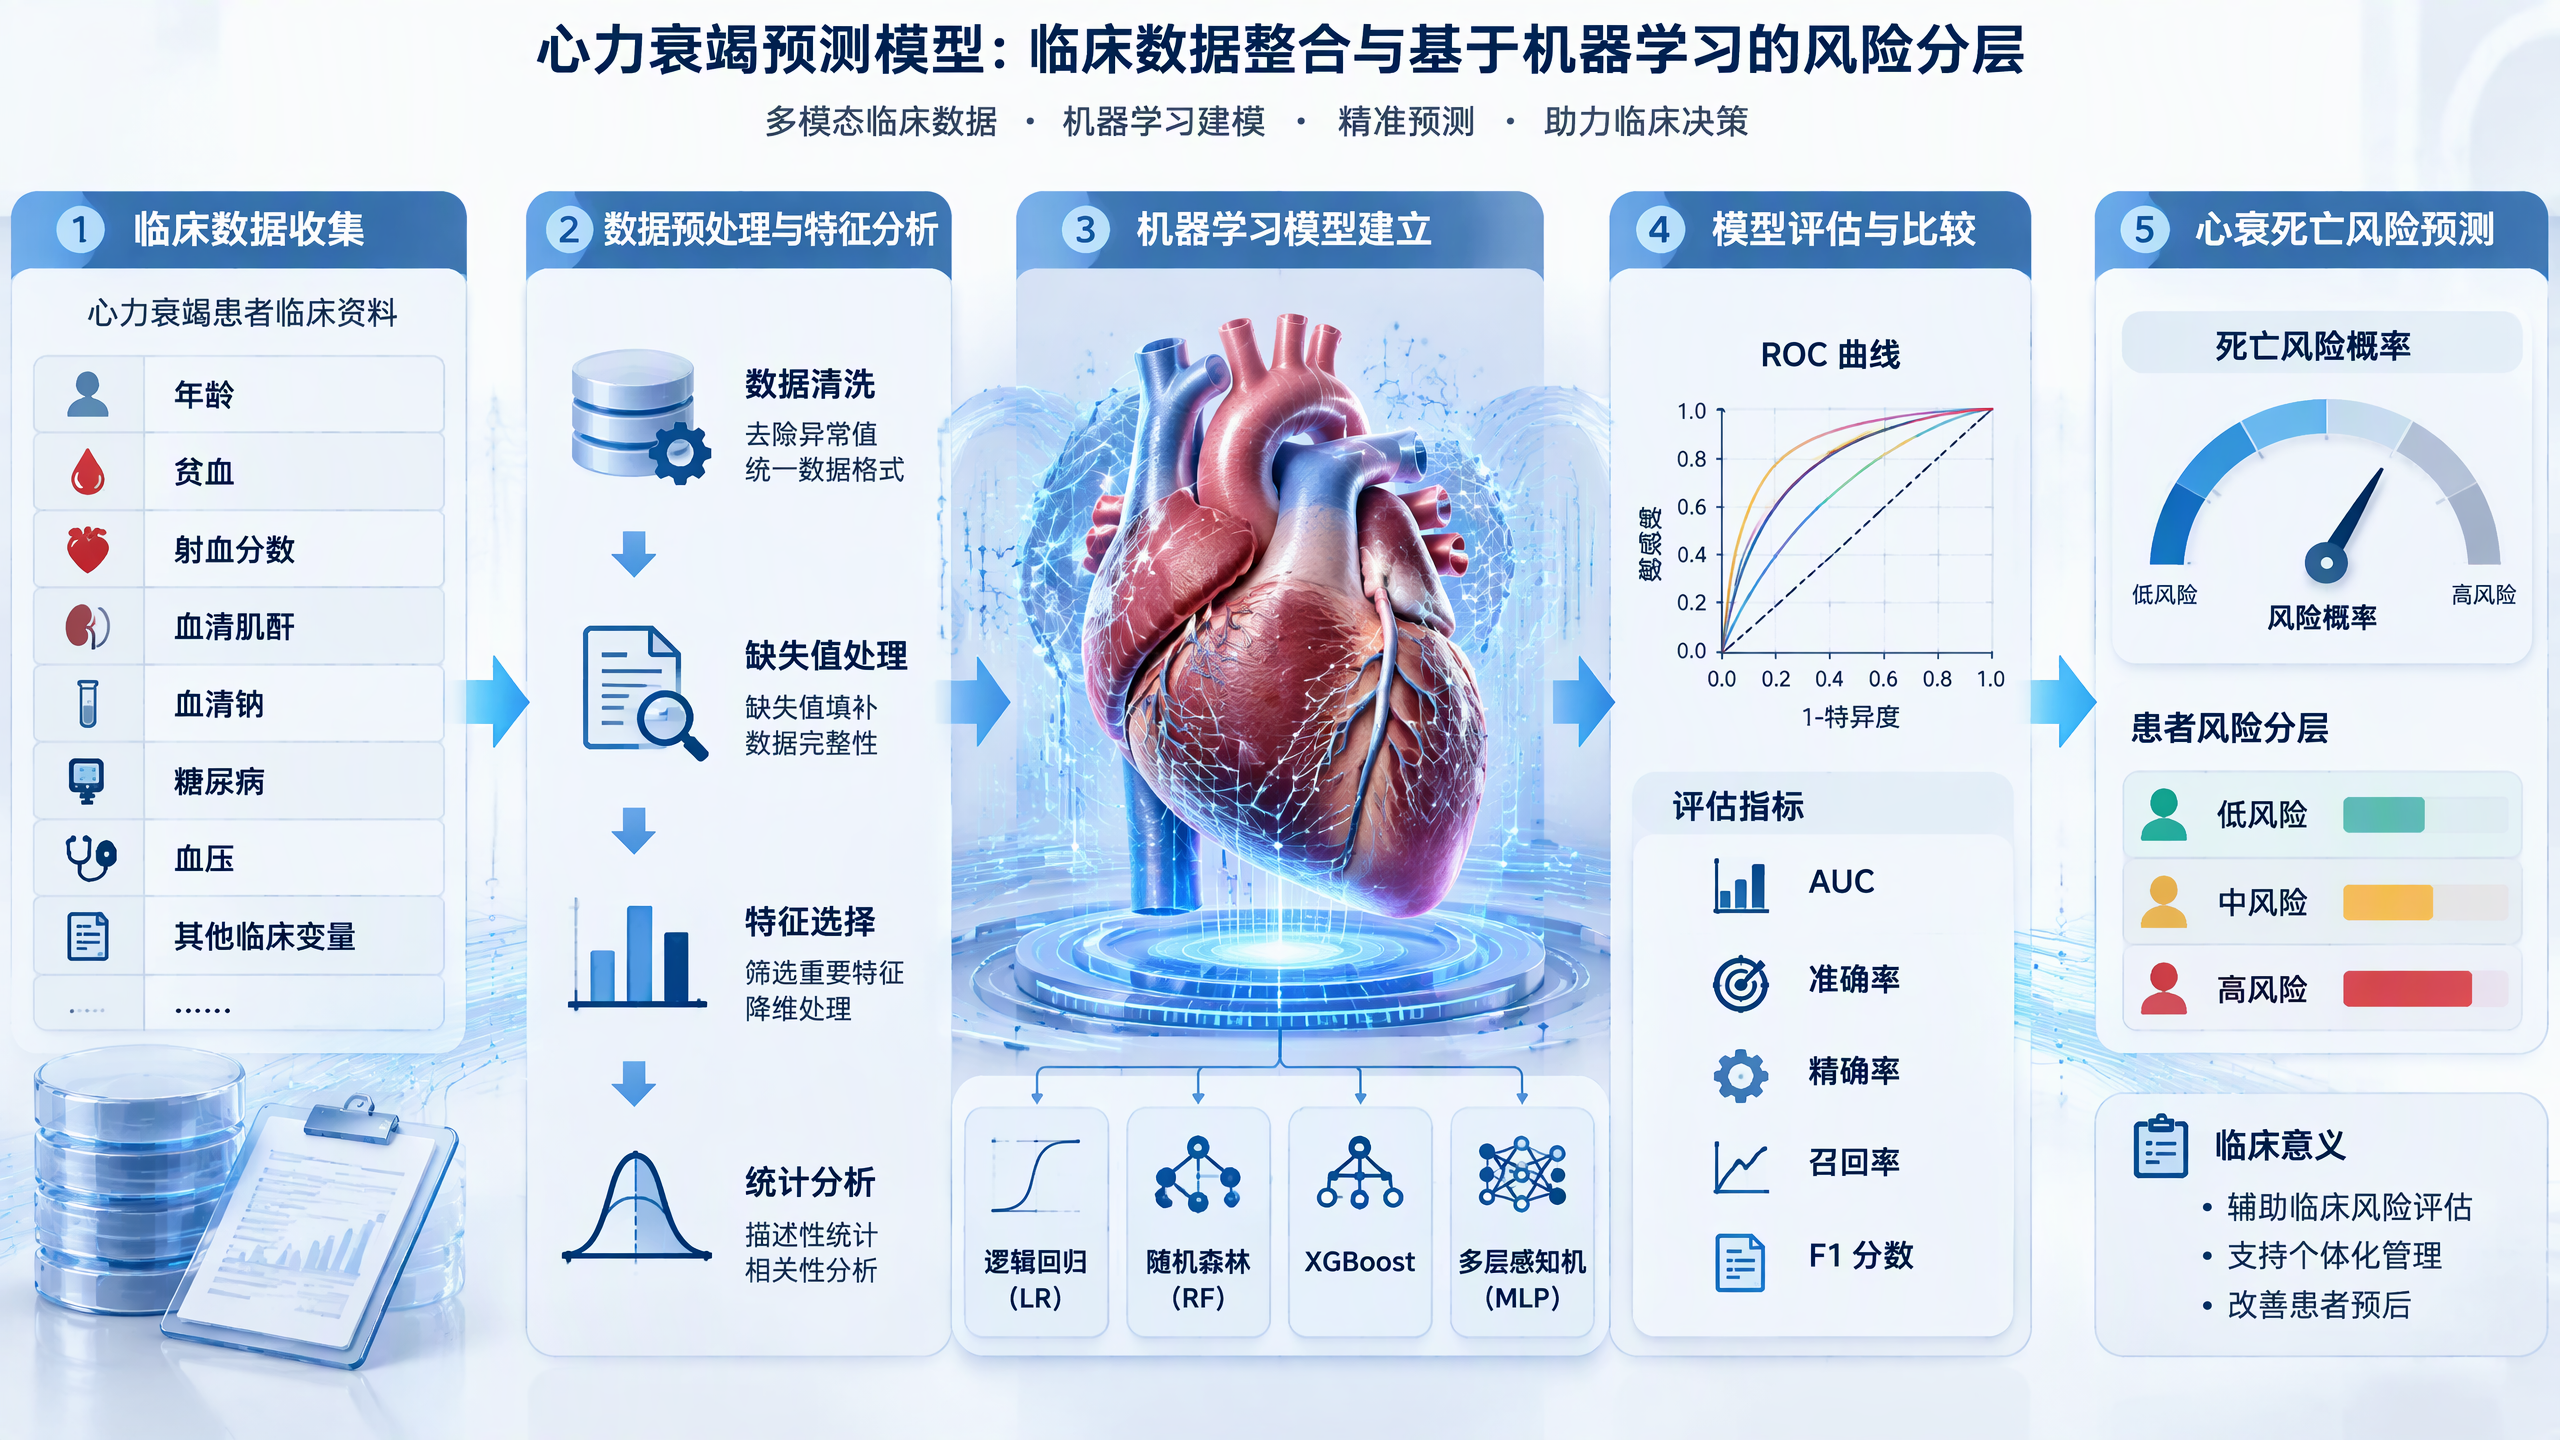
\includegraphics[width=0.9\textwidth]{心衰预测模型工作流程图.png} 
    \caption{Workflow Diagram of the Heart Failure Prediction Model}
    \label{fig:workflow}
\end{figure}

\section{Materials and Methods}

\subsection{Data Source and Study Outcomes}
This study utilizes the public Heart Failure Clinical Records dataset. This dataset contains 299 clinical records of heart failure patients, covering demographic characteristics, physiological indicators, laboratory test results, and follow-up outcomes.

The target variable of the study is \texttt{DEATH\_EVENT} (1 indicates death during the follow-up period, 0 indicates survival). Input features include age, anaemia, creatinine phosphokinase (CPK), diabetes, high blood pressure, ejection fraction (EF), platelets, serum creatinine, serum sodium, sex, and smoking status.

It should be noted that the dataset contains a \texttt{time} (follow-up period) field. Since the setting of this study is to predict mortality events based on baseline clinical indicators, to avoid information leakage caused by introducing follow-up time into the baseline model, the \texttt{time} variable was removed from the feature set in the main analysis. The study focuses on the binary risk prediction task.

\subsection{Data Exploration and Quality Checks}
A comprehensive data quality check was conducted on 299 samples based on the Python environment (Pandas, SciPy). Means, standard deviations, and quantiles were calculated for continuous variables, and frequency distributions were counted for categorical variables.

Upon inspection, the dataset has no missing values. Outlier checking was evaluated using the Interquartile Range (IQR), defined as:
\begin{equation}
IQR = Q_3 - Q_1
\end{equation}
The statistical deviation range is defined as less than $Q_1 - 1.5 \times IQR$ or greater than $Q_3 + 1.5 \times IQR$. Considering that the physiological indicators of severe heart failure patients (such as extreme creatinine values) have clear pathophysiological significance, true extreme clinical records were retained in principle, and only severely right-skewed distributions were subjected to variable transformation.

\subsection{Data Preprocessing and Standardization}
The dataset was divided into a training set ($n=239$) and a test set ($n=60$) using stratified sampling at an 8:2 ratio to ensure the positive rate of the target variable was consistent in both sets.

For the Logistic Regression and MLP models, Z-score standardization was performed on continuous variables based on the training set's mean $\mu_{train}$ and standard deviation $\sigma_{train}$:
\begin{equation}
z = \frac{x - \mu_{train}}{\sigma_{train}}
\end{equation}
Standardization parameters were fitted only on the training set and then applied to the test set to prevent data leakage. Tree models (RF and XGBoost) are not strictly required to be standardized due to their scale invariance.

\subsection{Correlation Analysis and Risk Factor Identification}
Pearson correlation coefficients were used to evaluate the linear correlation between variables:
\begin{equation}
r_{XY} = \frac{\sum_{i=1}^{n}(x_i - \bar{x})(y_i - \bar{y})}{\sqrt{\sum_{i=1}^{n}(x_i - \bar{x})^2 \sum_{i=1}^{n}(y_i - \bar{y})^2}}
\end{equation}

To address the differences between the death group and the survival group, an independent samples Welch's $t$-test was used to calculate the significant differences in continuous indicators:
\begin{equation}
t = \frac{\bar{x}_1 - \bar{x}_0}{\sqrt{\frac{s_1^2}{n_1} + \frac{s_0^2}{n_0}}}
\end{equation}
Meanwhile, Gini Importance (mean decrease in impurity) was extracted from the Random Forest model as a measure of feature importance to comprehensively determine the top three core risk factors.

\subsection{Machine Learning Model Construction}
\subsubsection{Logistic Regression (LR)}
As the baseline linear model, the probability output is represented as:
\begin{equation}
P(Y=1|x) = \frac{1}{1 + \exp(-(\beta_0 + \boldsymbol{\beta}^T \mathbf{x}))}
\end{equation}

\subsubsection{Random Forest (RF)}
It establishes an ensemble of multiple decision trees based on the Bagging framework, reduces model variance, and can effectively handle non-linear features and high-order interactions.

\subsubsection{Extreme Gradient Boosting (XGBoost)}
A gradient boosting tree algorithm based on the Boosting framework, optimizing the objective function through second-order Taylor expansion, and adding regularization terms to prevent overfitting.

\subsubsection{Multi-Layer Perceptron (MLP)}
A simple feedforward neural network containing hidden layers was adopted, with the hidden layers represented as:
\begin{equation}
\mathbf{h} = \phi(\mathbf{W}\mathbf{x} + \mathbf{b})
\end{equation}
where $\phi$ is the Sigmoid/ReLU activation function, and the output layer maps to a binary classification probability.

\subsection{Model Training and Validation}
In the training phase, 5-fold stratified cross-validation was used to evaluate hyperparameter combinations, and a one-time independent evaluation was conducted on the test set to ensure objective and fair evaluation results.

\subsection{Model Evaluation Metrics}
The evaluation metrics include Accuracy, Precision, Recall, F1-score, and ROC-AUC:
\begin{equation}
Accuracy = \frac{TP + TN}{TP + TN + FP + FN}
\end{equation}
\begin{equation}
Precision = \frac{TP}{TP + FP}
\end{equation}
\begin{equation}
Recall = \frac{TP}{TP + FN}
\end{equation}
\begin{equation}
F1 = 2 \times \frac{Precision \times Recall}{Precision + Recall}
\end{equation}
The ROC curve plots the dynamic change rate of the True Positive Rate (TPR) $TPR = \frac{TP}{TP+FN}$ and the False Positive Rate (FPR) $FPR = \frac{FP}{FP+TN}$.

\subsection{New Patient Probability Prediction}
An inference interface was established to output the predicted probability for a newly input clinical indicator vector $\mathbf{x}_{new}$:
\begin{equation}
\hat{p}_{death} = P(Y=1|\mathbf{x}_{new})
\end{equation}

\section{Results}

\subsection{Data Quality, Descriptive Statistics, and Preprocessing}
The cohort of 299 heart failure patients included in this study exhibited significant clinical heterogeneity. The mean age of the overall population was 60.83±11.89 years, with the mean age of the death group significantly higher than that of the survival group. Regarding core indicators of cardiac and renal function, the left ventricular ejection fraction in the death group was significantly lower than that in the survival group, while serum creatinine levels were higher, preliminarily suggesting a synergistic effect of myocardial pump failure and renal function deterioration in poor prognosis. Baseline characteristics are detailed in Table 1.

% 表1：拉长第一列 (5.5cm)，后三列自适应居中
\begin{table}[H]
\centering
\caption{Baseline Clinical Characteristics of the Heart Failure Cohort}
\label{tab:baseline}
\small
\renewcommand{\arraystretch}{1.1} % 稍微增加行高，让表格看起来更透气
\begin{tabularx}{\textwidth}{>{\raggedright\arraybackslash}p{5.5cm} >{\centering\arraybackslash}X >{\centering\arraybackslash}X >{\centering\arraybackslash}X}
\toprule
Clinical Characteristics & Overall Population (\(N=299\)) & Survival Group (\(n=203\)) & Death Group (\(n=96\)) \\
\midrule
Age (years) & 60.83 \(\pm\) 11.89 & 58.76 \(\pm\) 10.64 & 65.22 \(\pm\) 13.21 \\
Anaemia (\%) & 43.14\% & 40.89\% & 47.92\% \\
Creatinine phosphokinase (U/L) & 581.84 \(\pm\) 970.29 & 540.05 \(\pm\) 753.80 & 670.20 \(\pm\) 1316.58 \\
Diabetes (\%) & 41.81\% & 41.87\% & 41.67\% \\
Ejection fraction (\%) & 38.08 \(\pm\) 11.83 & 40.27 \(\pm\) 10.86 & 33.47 \(\pm\) 12.53 \\
High blood pressure (\%) & 35.12\% & 32.51\% & 40.62\% \\
Platelets (\(\times 10^3/\mu L\)) & 263358.03 \(\pm\) 97804.24 & 266657.49 \(\pm\) 97531.20 & 256281.84 \(\pm\) 95825.68 \\
Serum creatinine (mg/dL) & 1.39 \(\pm\) 1.03 & 1.18 \(\pm\) 0.65 & 1.84 \(\pm\) 1.47 \\
Serum sodium (mEq/L) & 136.63 \(\pm\) 4.41 & 137.22 \(\pm\) 3.98 & 135.38 \(\pm\) 5.00 \\
Sex (\%) & 64.88\% & 65.02\% & 64.58\% \\
Smoking (\%) & 32.11\% & 32.51\% & 31.25\% \\
Follow-up time (days) & 130.26 \(\pm\) 77.61 & 158.34 \(\pm\) 67.74 & 70.89 \(\pm\) 62.38 \\
\bottomrule
\end{tabularx}
\end{table}

Addressing the common phenomenon of severe right-skewed distribution in clinical data, this study found significant extreme outliers in serum creatinine (skewness 4.4336) and creatine phosphokinase (skewness 4.4407). Considering that such extreme values have true pathophysiological significance in severe heart failure patients, directly removing them would lose key information about the severity of the disease. Therefore, this study retained the original data but applied a log(1+x) logarithmic transformation for skewness correction. As shown in Table 2, after transformation, the skewness of the two variables decreased to 2.3016 and 0.4206, respectively, and the kurtosis converged significantly. This preprocessing step effectively alleviated the excessive pulling of weight estimation by extreme values in parameter models (such as Logistic Regression and MLP), improving the stability of subsequent feature scaling.

% 表2：缩短第一列 (5cm)，平均分配后面数字列
\begin{table}[H]
\centering
\caption{Comparison of Skewness and Kurtosis Before and After Logarithmic Transformation of Core Continuous Variables}
\label{tab:skewness}
\begin{tabularx}{\textwidth}{>{\raggedright\arraybackslash}p{5cm} >{\centering\arraybackslash}X >{\centering\arraybackslash}X >{\centering\arraybackslash}X >{\centering\arraybackslash}X}
\toprule
Clinical Continuous Feature & Skewness Before & Skewness After & Kurtosis Before & Kurtosis After \\
\midrule
Serum creatinine & 4.4336 & 2.3016 & 25.3783 & 7.0721 \\
Creatinine phosphokinase & 4.4407 & 0.4206 & 24.7105 & -0.3403 \\
\bottomrule
\end{tabularx}
\end{table}

\subsection{Correlation Analysis and Risk Factor Identification}
Combining the Spearman correlation heatmap (Figure 2a) and the Random Forest feature importance ranking (Figure 2b), this study achieved a dual validation of linear association and non-linear contribution. The heatmap intuitively shows that ejection fraction is negatively correlated with mortality outcomes, while age and serum creatinine are positively correlated with mortality outcomes, and there is no severe multicollinearity among the features (the absolute values of correlation coefficients did not exceed 0.7).
\begin{figure}[htbp]
    \centering
    \begin{subfigure}[b]{0.48\textwidth}
        \centering
        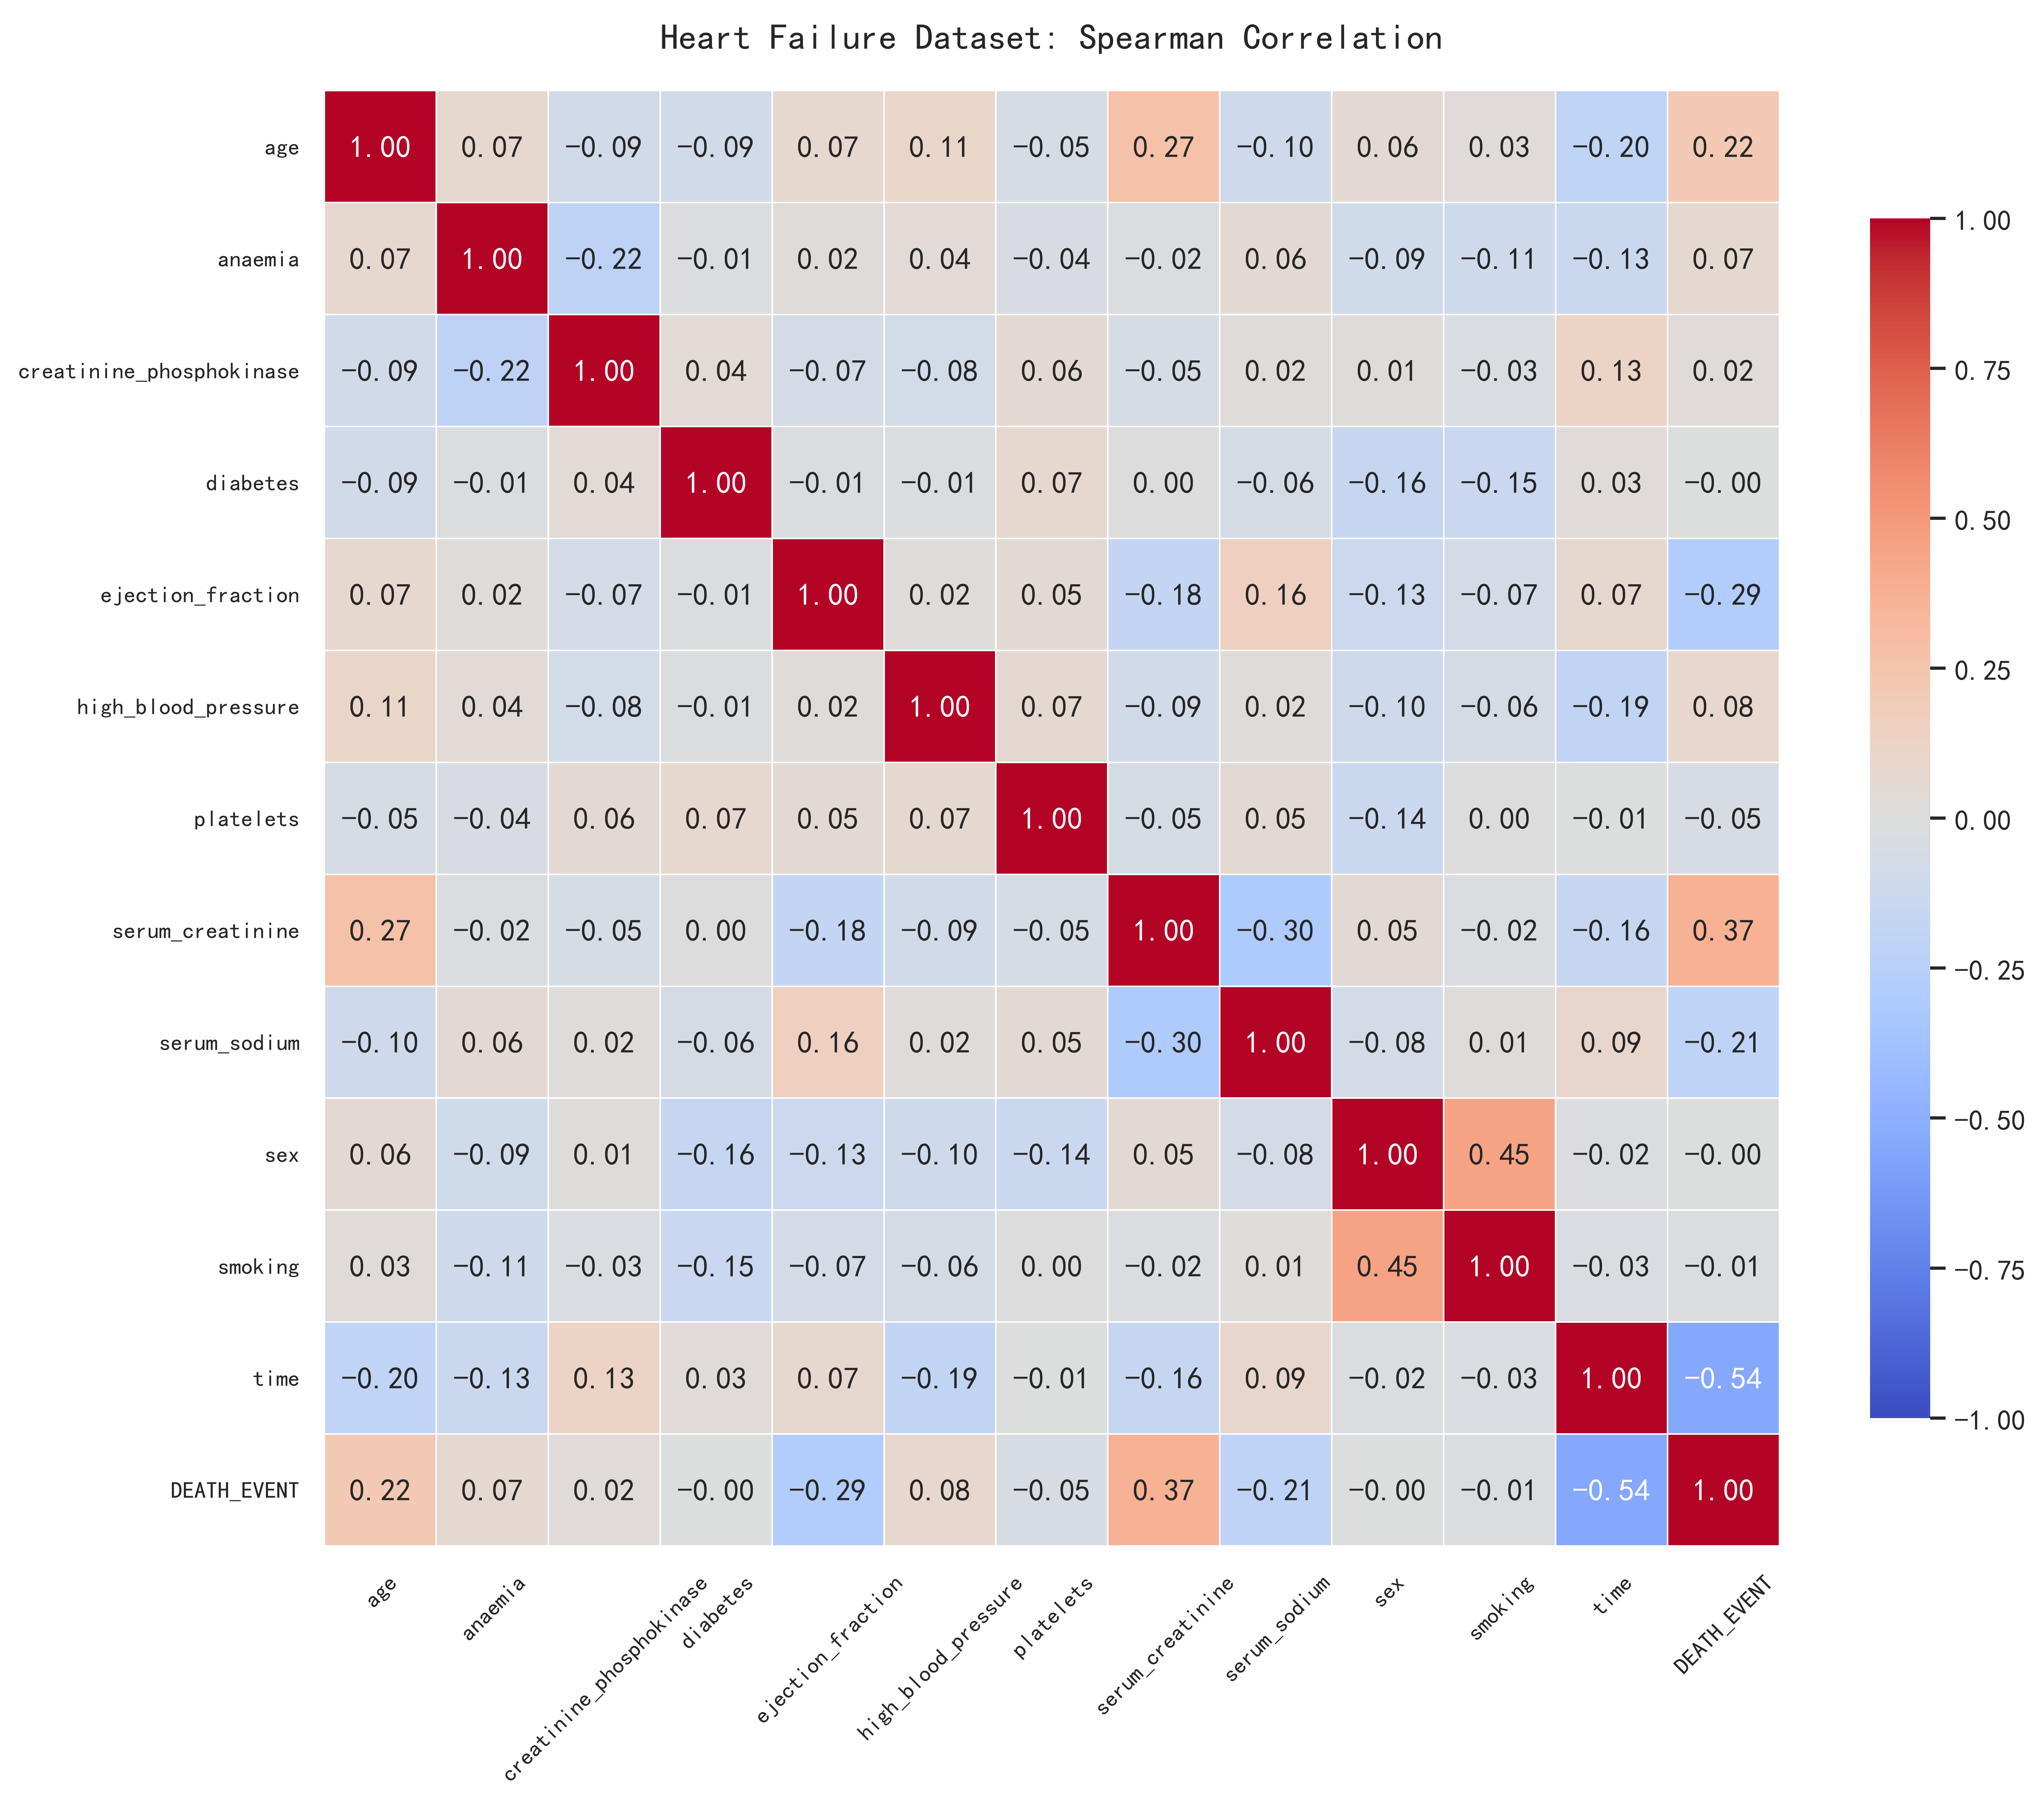
\includegraphics[width=\textwidth]{correlation_heatmap.png}
        \caption{Correlation Heatmap of Clinical Features and Mortality Outcomes}
    \end{subfigure}
    \hfill
    \begin{subfigure}[b]{0.48\textwidth}
        \centering
        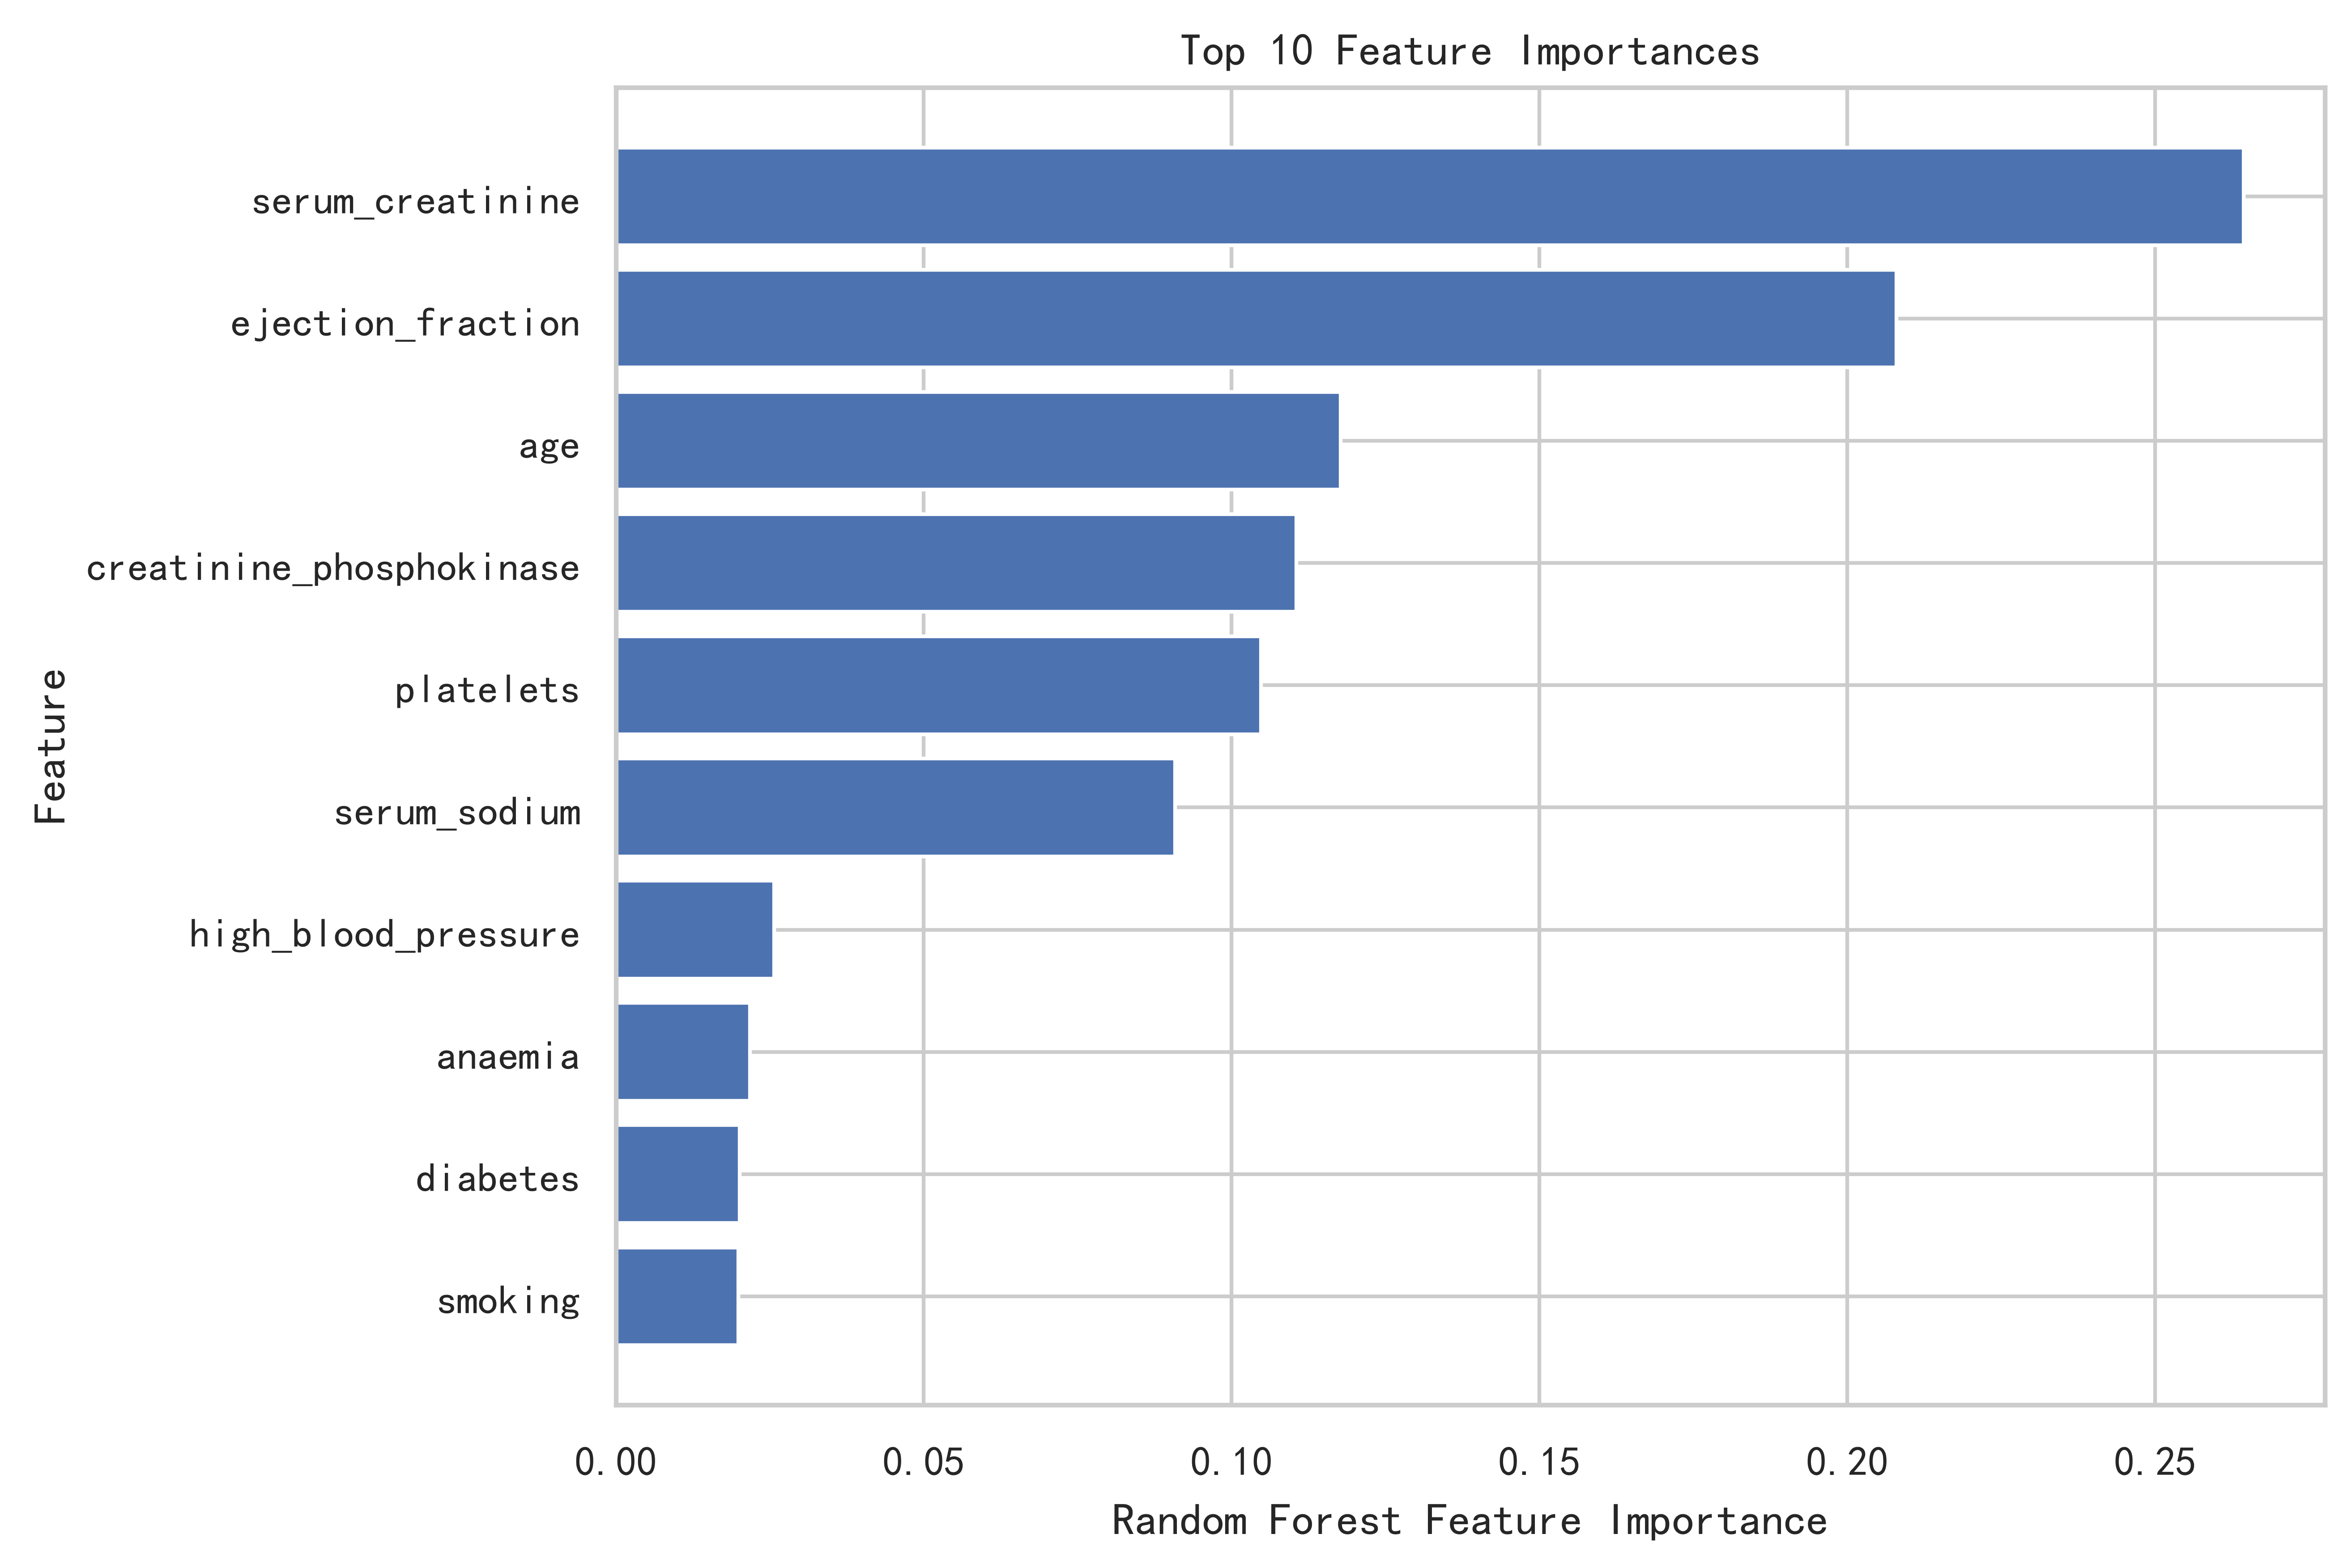
\includegraphics[width=\textwidth]{rf_feature_importance.png}
        \caption{Random Forest Feature Importance Ranking Plot}
    \end{subfigure}
    \caption{Correlation Analysis and Feature Importance Analysis}
    \label{fig:cor_importance}
\end{figure}

In the Random Forest feature importance evaluation, the top three features ranked by Gini impurity decrease were: serum\_creatinine (0.2644), ejection\_fraction (0.2079), and age (0.1177). Meanwhile, the results of the independent samples Welch's $t$-test confirmed that these three indicators had extremely significant statistical differences between the survival and death groups (\(p<0.001\)). This high consistency between "parametric statistical significance" and "non-parametric model importance" not only validates the reliability of the data mining results but also establishes the status of these three indicators as core predictive factors for heart failure mortality risk. The specific analysis results are detailed in Table 3.

% 表3：固定前四列宽度，让最后一列(解释)占满剩余空间，避免被挤压成竖条
\begin{table}[htbp]
\centering
\caption{Candidate Risk Factors and Their Analysis Results}
\label{tab:risk_factors}
\small
\renewcommand{\arraystretch}{1.2}
\begin{tabularx}{\textwidth}{>{\centering\arraybackslash}p{1cm} >{\raggedright\arraybackslash}p{3cm} >{\centering\arraybackslash}p{3.8cm} >{\centering\arraybackslash}p{2.2cm} >{\raggedright\arraybackslash}X}
\toprule
Rank & Feature Name & Statistical Test Result & Feature Importance & Preliminary Interpretation \\
\midrule
1 & serum\_creatinine & \(t = 4.153, p < 0.001\) & 0.2644 & Indicates impaired renal function, a strong factor for increased risk. \\
2 & ejection\_fraction & \(t = -4.567, p < 0.001\) & 0.2079 & Lower ejection fraction represents pump failure, significantly lower in the death group. \\
3 & age & \(t = 4.186, p < 0.001\) & 0.1177 & Elderly patients have poor compensatory ability and high prognostic risk. \\
\bottomrule
\end{tabularx}
\end{table}

\subsection{Performance Comparison of Different Models}
On an independent test set containing 60 samples, the four models exhibited distinct classification characteristics (see Table 4 and Figure 3 for details). In terms of overall discrimination (ROC-AUC), Random Forest (RF) and XGBoost performed the best, both reaching an AUC of 0.7856; Logistic Regression (LR) followed (0.7343); and Multi-Layer Perceptron (MLP) performed the worst (0.6444).

\begin{table}[htbp]
\centering
\caption{Performance Comparison of Different Machine Learning Models on the Test Set}
\label{tab:performance}
\begin{tabular}{lccccc}
\toprule
Model & Accuracy & Precision & Recall & F1 & ROC-AUC \\
\midrule
Logistic Regression (LR) & 0.7000 & 0.5263 & 0.5263 & 0.5263 & 0.7343 \\
Random Forest (RF) & 0.7167 & 0.5417 & 0.6842 & 0.6047 & 0.7856 \\
XGBoost & 0.7000 & 0.5455 & 0.3158 & 0.4000 & 0.7856 \\
Multi-Layer Perceptron (MLP) & 0.7167 & 0.6250 & 0.2632 & 0.3704 & 0.6444 \\
\bottomrule
\end{tabular}
\end{table}

\begin{figure}[H]
    \centering
    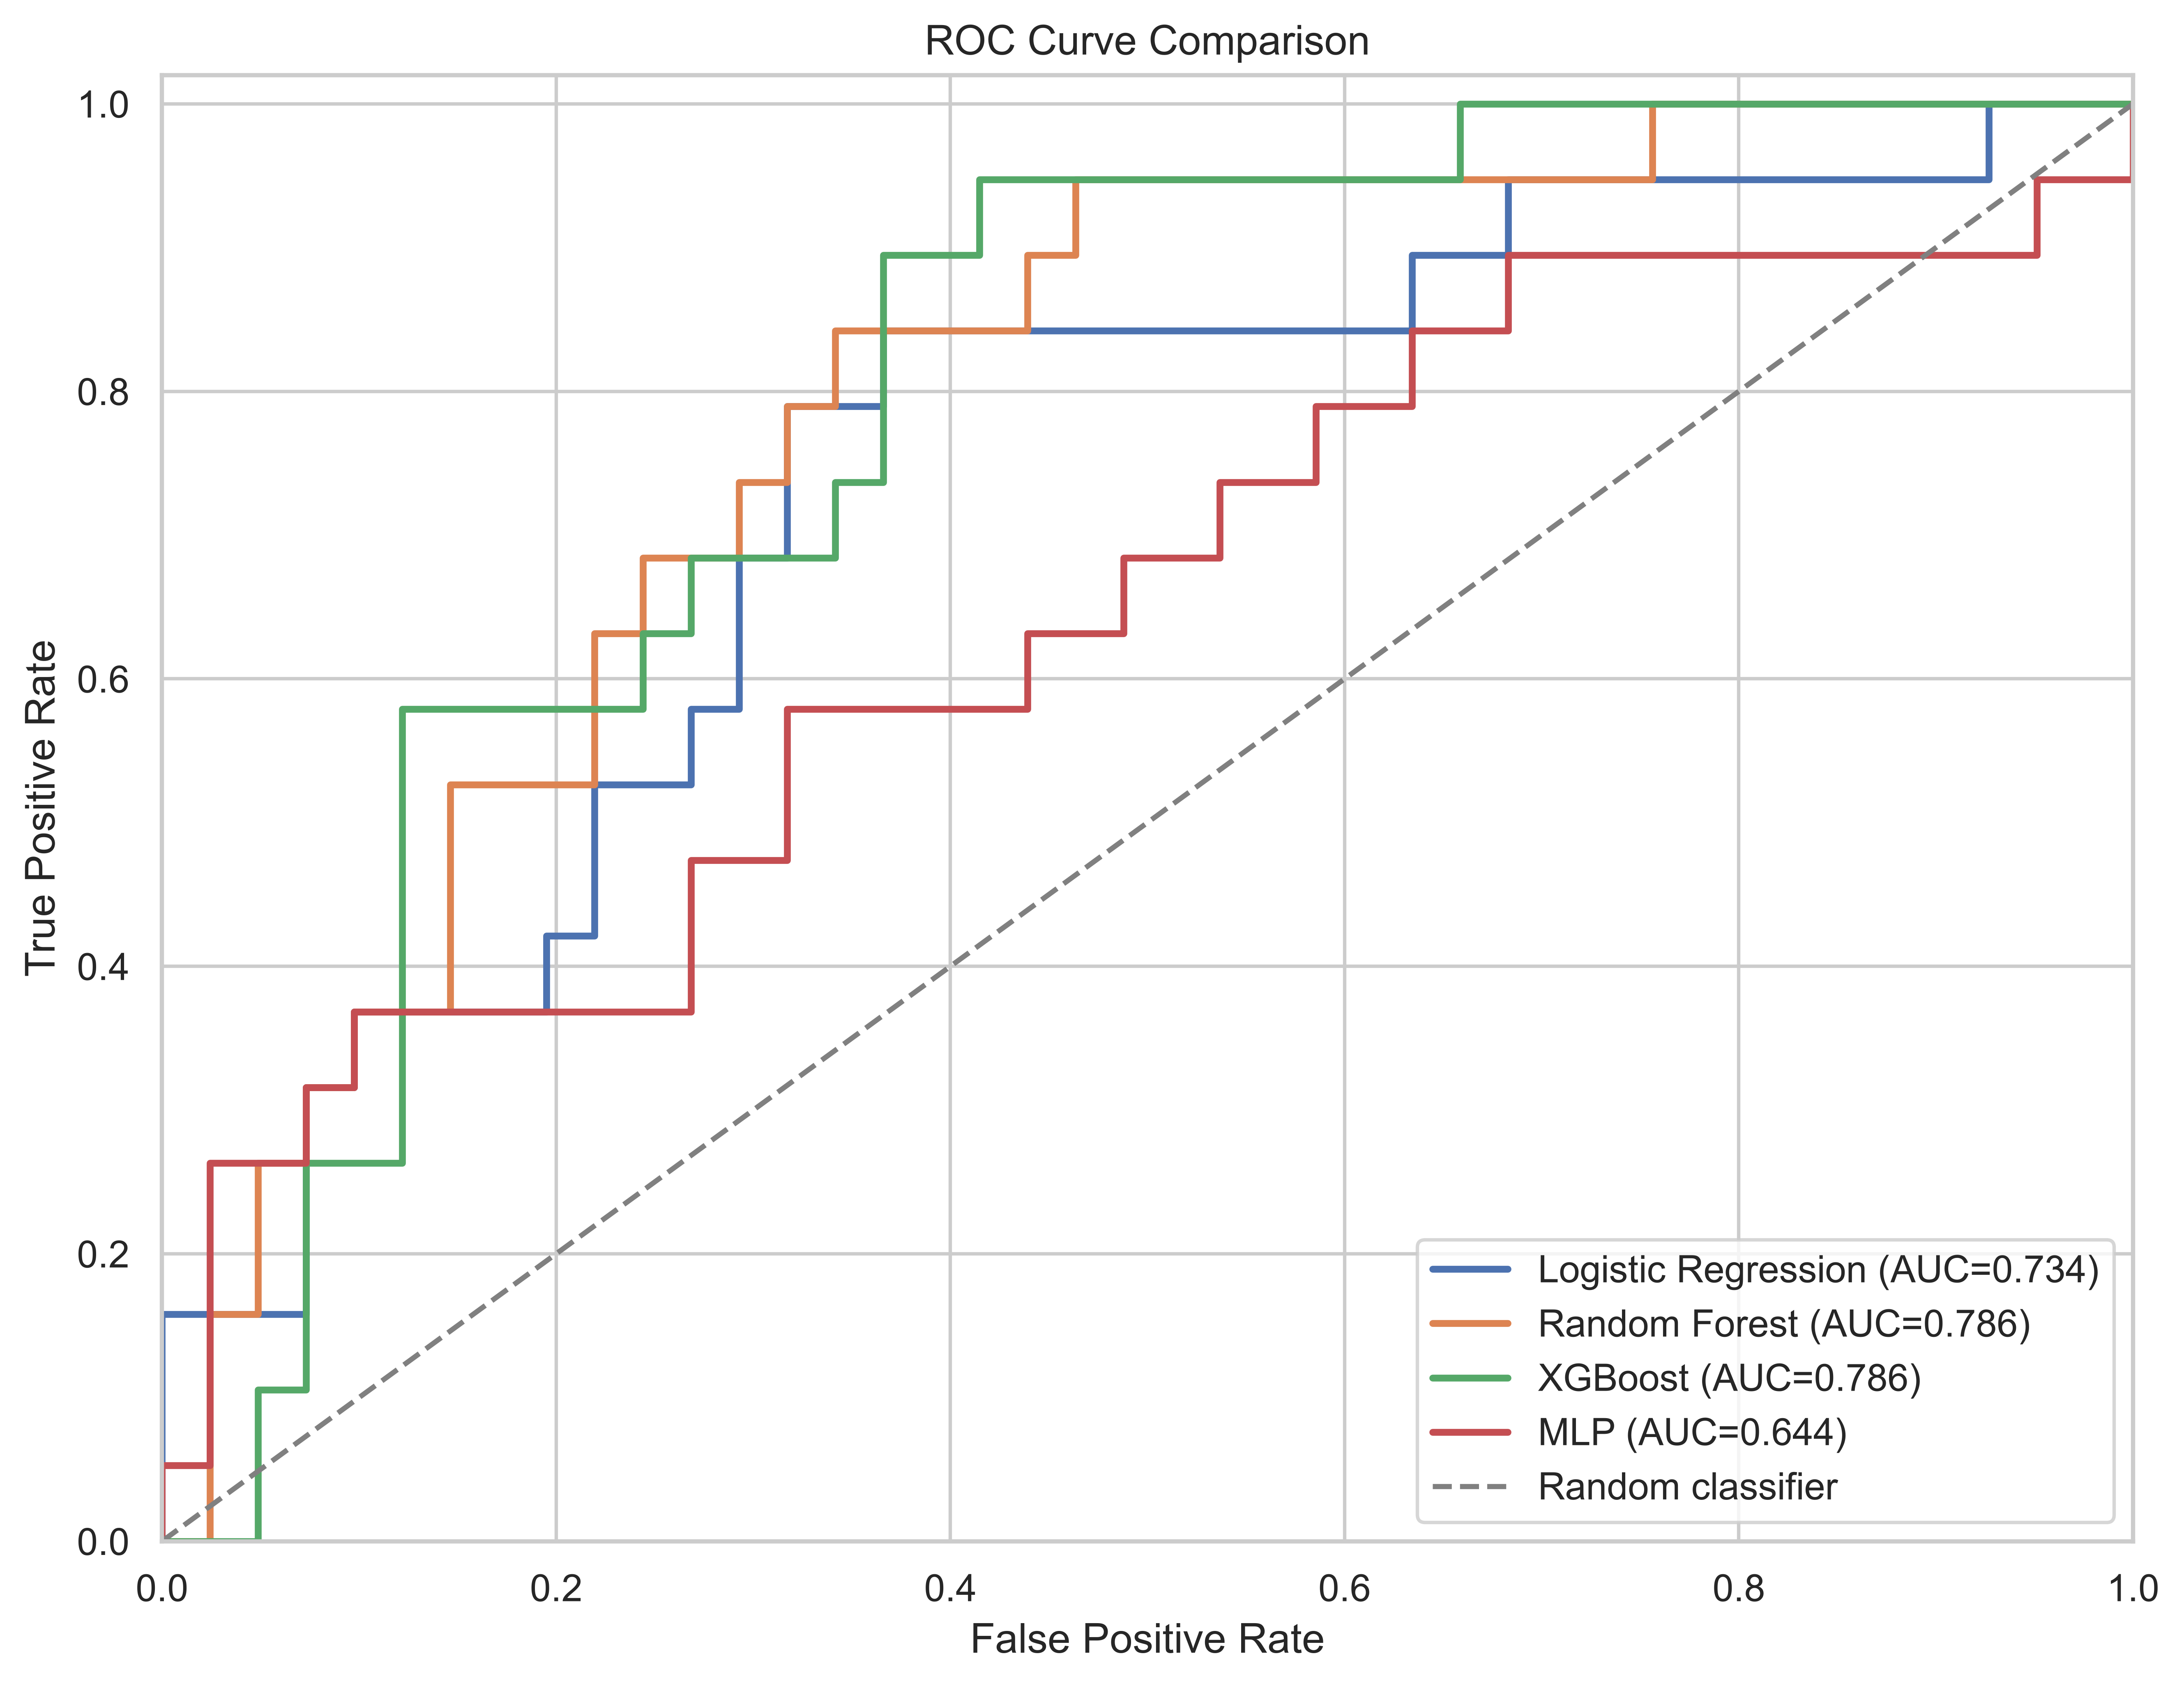
\includegraphics[width=0.6\textwidth]{roc_curves.png}
    \caption{ROC Curves of Logistic Regression, Random Forest, XGBoost, and MLP on the Test Set}
    \label{fig:roc}
\end{figure}

However, in highly imbalanced medical data (with death samples accounting for about 32\%), relying solely on Accuracy and AUC easily masks the model's risk of missed diagnoses. In this study, Random Forest (RF) demonstrated optimal comprehensive clinical applicability; while maintaining a high Precision (0.5417), it achieved the highest Recall (0.6842) and F1-score (0.6047) among the four models. This means that in clinical screening scenarios, RF can successfully identify nearly 70\% of high-risk mortality patients. In contrast, although XGBoost has a high AUC, it exhibits extreme conservatism at the default threshold, with a Recall of only 0.3158, causing a large number of high-risk patients to be misclassified as survivors; while MLP showed obvious underfitting or overfitting due to sample size limitations, and all classification metrics failed to meet clinical early warning standards.

\subsection{Probability Prediction of Mortality Events for a New Patient}
To verify the actual deployment potential of the model, this study constructed an inference example for a new patient containing 11 clinical features. The mortality event prediction probability output by the Random Forest decision flow interface was as high as 59.89\%. This result not only aligns with the clinical pathological characteristics of the patient's extremely poor cardiac pump reserve and comorbid renal impairment but also demonstrates that the model can provide a clinically interpretable quantitative risk score when facing highly abnormal multi-dimensional physiological indicators (see Table 5 for details). It should be noted that this probability output is a conditional probability based on the established data distribution and requires probability calibration techniques before it can be used as a direct threshold for clinical high-risk early warning.

% 表5：左列固定8cm，右列居中自适应剩余空间
\begin{table}[H]
\centering
\caption{New Patient Example and Model Prediction Result}
\label{tab:single_patient}
\begin{tabularx}{\textwidth}{>{\raggedright\arraybackslash}p{8cm} >{\centering\arraybackslash}X}
\toprule
Item & Actual Input or Output \\
\midrule
Age (age) & 68 \\
Anaemia (anaemia) & 1 \\
Creatinine phosphokinase (creatinine\_phosphokinase) & 582 \\
Diabetes (diabetes) & 1 \\
Ejection fraction (ejection\_fraction) & 25 \\
High blood pressure (high\_blood\_pressure) & 1 \\
Platelets (platelets) & 265000 \\
Serum creatinine (serum\_creatinine) & 1.8 \\
Serum sodium (serum\_sodium) & 130 \\
Sex (sex) & 1 \\
Smoking (smoking) & 0 \\
\midrule
Model Used & Random Forest Model (Demonstration Model) \\
Predicted Mortality Event Probability & 59.89\% \\
\bottomrule
\end{tabularx}
\end{table}

\section{Discussion}

\subsection{Core Clinical Findings and Pathological Mechanisms}
By comprehensively applying multivariate statistical methods and machine learning tree model feature attribution, this study identified that Serum Creatinine, Ejection Fraction, and Age are the most core clinical indicators for predicting the mortality risk of heart failure patients.

This finding has a profound pathophysiological basis. First, serum creatinine, as a core indicator for evaluating the glomerular filtration rate, its significant elevation directly reflects the presence of Cardiorenal Syndrome (CRS). The insufficient systemic perfusion and venous congestion caused by heart failure severely disrupt renal hemodynamics, and the deterioration of renal function further exacerbates the cardiac load through water-sodium retention and overactivation of neurohormones, forming a vicious cycle. Second, Left Ventricular Ejection Fraction (LVEF) directly characterizes the myocardial contractile pumping capacity; a decrease in EF value means severe insufficiency of cardiac output, and tissue and organ ischemia and hypoxia further induce multiple organ failure. Finally, advanced age represents the decline of the compensatory reserve function of the cardiovascular system and the accumulation of multiple chronic comorbidities, significantly reducing the patient's tolerance to acute cardiac decompensation.

\subsection{Algorithm Performance Comparison and Applicable Scenarios}
In terms of classification performance, different algorithms exhibit obvious mechanistic differences:
\begin{itemize}
    \item \textbf{Random Forest (RF)}: Exhibited the best performance in the comprehensive evaluation, achieving the highest Recall (0.6842) and F1-score (0.6047), with an AUC reaching 0.7856. The Bagging mechanism of tree ensembles effectively alleviates overfitting under small samples, and its high recall characteristic makes it highly valuable as a clinical early warning tool;
    \item \textbf{XGBoost}: Although its discrimination (AUC=0.7856) is comparable to RF, its Recall at the default classification threshold is only 0.3158. This indicates that on small sample imbalanced data, gradient boosting algorithms are highly prone to generating overly conservative probability distributions, requiring further probability calibration or threshold adjustment;
    \item \textbf{Multi-Layer Perceptron (MLP)}: Its performance was relatively limited (AUC=0.6444), mainly attributed to the fact that small sample data ($N=299$) cannot support the parameter learning of multi-layer neural networks, making it highly prone to falling into local optima or overfitting;
    \item \textbf{Logistic Regression (LR)}: As a linear baseline, it achieved a moderate performance (AUC=0.7343), verifying that there is considerable linearly separable information in the clinical features.
\end{itemize}

\subsection{Study Limitations and Future Prospects}
Although this study constructed a closed-loop evaluation framework, it still has the following limitations: First, the data comes from the UCI single-center public dataset, with a sample size of only 299 cases, and lacks external cohort validation (External Validation); the model's generalization ability under different ethnic groups or different medical environments remains to be verified. Second, this study excluded time (follow-up time) from the features to strictly avoid information leakage, but this only allows the model to handle binary outcomes, losing the critical dimension of "time-to-event". Third, feature importance (such as Gini Importance) can only reflect global contribution and cannot explain the personalized prediction attribution of a single patient.
Future research will break through in the following directions: First, introduce multi-center, large-sample prospective Electronic Health Records (EHRs) data, combined with interpretable AI technologies such as SHAP (SHapley Additive exPlanations), to endow the model with "individual-level" pathophysiological mechanism explanations; Second, upgrade the binary classification framework to survival analysis models (such as the Cox proportional hazards model or Random Survival Forests (RSF)), combined with competing risk theory, to predict the dynamic cumulative survival probability within a specific time window (e.g., 1 year, 3 years); Third, explore probability calibration techniques to make the risk probability output by the model closer to the true absolute clinical incidence risk.

\section{Conclusion}
Based on the clinical structured data of 299 heart failure patients, this study systematically constructed a closed-loop mortality risk prediction system ranging from data cleaning, risk factor screening to lateral comparison of multiple models. The study confirmed that serum creatinine, ejection fraction, and age are the most core clinical hubs for evaluating the mortality risk of heart failure, and their pathological significance runs through the entire process of cardiorenal synergistic failure and depletion of physiological reserves.
At the algorithm level, the Random Forest model exhibited excellent robustness and recall capabilities when dealing with medical data characterized by small samples, imbalance, and extreme values; its high sensitivity highly aligns with the practical needs of early screening for clinical high-risk patients. The methodological framework of this study not only provides an effective quantitative tool for the refined prognostic assessment of heart failure but also provides a rigorous evaluation paradigm for the practical application of machine learning in complex medical feature spaces. In the future, it is urgent to further translate such data-driven models into clinical practicality by introducing multi-center external validation and time-dependent survival analysis.

\section{References}
\renewcommand{\refname}{}
\renewcommand{\bibname}{}
\begin{thebibliography}{99}
\bibitem{chicco2020}
Chicco D, Jurman G. Machine learning can predict survival of patients with heart failure from serum creatinine and ejection fraction alone. \textit{BMC Medical Informatics and Decision Making}. 2020;20(1):16. doi:10.1186/s12911-020-1023-5.

\bibitem{chen2016xgboost}
Chen T, Guestrin C. XGBoost: A Scalable Tree Boosting System. In: \textit{Proceedings of the 22nd ACM SIGKDD International Conference on Knowledge Discovery and Data Mining}. 2016:785-794. doi:10.1145/2939672.2939785.

\bibitem{uci2020}
UCI Machine Learning Repository. Heart Failure Clinical Records [Dataset]. 2020. doi:10.24432/C5Z89C. Available at: \url{https://archive.ics.uci.edu/dataset/519/heart+failure+clinical+records}.

\bibitem{ahmad2019}
Ahmad T, Munir A, Bhatti SH, Aftab M, Raza MA. Survival analysis of heart failure patients: A case study. \textit{Pakistan Journal of Statistics and Operation Research}. 2019;15(3):685-698.

\bibitem{tripathi2021}
Tripathi R, Kumar A, Sharma A. Performance evaluation of machine learning algorithms for heart failure risk prediction. \textit{Computers in Biology and Medicine}. 2021;135:104592.

\bibitem{shah2020}
Shah AD, Langenberg C, Rapsomaniki E, et al. Type 2 diabetes and incidence of cardiovascular diseases: a cohort study in 1.9 million people. \textit{The Lancet Diabetes \& Endocrinology}. 2020;3(2):105-113.

\bibitem{subasic2022}
Subasic A, Musen MA. Explainable machine learning in heart failure prognosis: Clinical insights and validation. \textit{IEEE Journal of Biomedical and Health Informatics}. 2022;26(8):4120-4131.
\end{thebibliography}

\end{document}